\documentclass[12pt]{article}

\usepackage{amsmath,amsthm,amsfonts,amssymb,amsxtra}
\usepackage{pgf,tikz}
\usetikzlibrary{arrows}
\renewcommand{\theenumi}{(\alph{enumi})} 
\renewcommand{\labelenumi}{\theenumi}

\pagestyle{empty}
\setlength{\textwidth}{7in}
\setlength{\oddsidemargin}{-0.5in}
\setlength{\topmargin}{-1.0in}
\setlength{\textheight}{9.5in}

\newtheorem{problem}{Problem}

\begin{document}

\noindent{\large\bf MATH 122}\hfill{\large\bf Second Midterm.}\hfill{\large\bf
  Spring 2012}\hfill{\large\bf Page 1/5}\hrule

\bigskip
\begin{center}
  \begin{tabular}{|ll|}
    \hline & \cr
    {\bf Name: } & \makebox[12cm]{\hrulefill}\cr & \cr
    {\bf 4-digit code:} & \makebox[12cm]{\hrulefill}\cr & \cr
    \hline
  \end{tabular}
\end{center}
\begin{itemize}
\item Write your name and the last 4 digits of your SSN in the space provided above.
\item The test has five (5) pages, including this one.
\item For multiple-choice questions, circle the answer you select.  On
  the other problems, you should enter your answer in the box(es)
  provided. 
\item Show sufficient work to justify all answers unless otherwise
  stated in the problem.  Correct answers with inconsistent work may
  not be given credit. 
\item Credit for each problem is given at the right of each problem
  number. 
\item No books or notes may be used on this test.  Calculators are
  allowed, provided they don't have a computer algebra system.
\end{itemize}
\hrule

\begin{center}
  \begin{tabular}{|c|c|c|}
    \hline
    &&\cr
    {\large\bf Page} & {\large\bf Max} & {\large\bf Points} \cr
    &&\cr
    \hline
    &&\cr
    {\Large 2} & \Large 30 & \cr
    &&\cr
    \hline
    &&\cr
    {\Large 3} & \Large 20 & \cr
    &&\cr
    \hline
    &&\cr
    {\Large 4} & \Large 20 & \cr
    &&\cr
    \hline
    &&\cr
    {\Large 5} & \Large 30 & \cr
    &&\cr
    \hline\hline
    &&\cr
    {\large\bf Total} & \Large 100 & \cr
    &&\cr
    \hline
  \end{tabular}
\end{center}
\newpage

%%%%%%%%%%%%%%%%%%%%%%%%%%%%%%%%%%%%% Page 2
\noindent{\large\bf MATH 122}\hfill{\large\bf Second Midterm.}\hfill{\large\bf
  Spring 2012}\hfill{\large\bf Page 2/5}\hrule

\bigskip
{\problem[10 pts] \em The quantity of ozone in the upper atmosphere, $Q$, is
decaying exponentially at a continuous rate of 0.2\% per year.  What is the half-life of ozone in the upper atmosphere?}
\vspace{4.5cm}
\begin{flushright}
  \begin{tikzpicture}
    \draw (0cm,-0.2cm) rectangle (5cm,1.2cm);
  \end{tikzpicture}
\end{flushright}
\hrule
{\problem[10 pts] \em If $g(t)=t^2$ and $f(t)=t+2$, then $f\big( g(t) \big)$ is:
\begin{enumerate}
\item $t^2+2$
\item $t^2+4$
\item $t^2+2t+4$

\noindent\begin{tikzpicture}
    \draw (0cm,0cm) node{None of the above!  The correct answer is };
    \draw (4cm,-0.5cm) rectangle (9cm,0.5cm); \end{tikzpicture}
\end{enumerate}
\hrule
{\problem[10 pts] \em For the function $f$ represented below, graph $2+f(x)$ in the same coordinate axes.}
\begin{center}
\begin{tikzpicture}
\draw[very thin,color=gray,step=0.5] (-1.9,-0.9) grid (4.9,3.9);
\draw[->,very thick] (-2.2,0) -- (5.2,0) node[right] {$x$};
\draw[->,very thick] (0,-1.2) -- (0,4.2) node[above] {$y$};
\draw[thick] (-1,-0.9) cos (-0.5,-0.5) sin (1,1) cos (3,0) sin (4,-0.5) cos (5,0);
\end{tikzpicture}
\end{center}
\newpage

%%%%%%%%%%%%%%%%%%%%%%%%%%%%%%%%%%%%% Page 3
\noindent{\large\bf MATH 122}\hfill{\large\bf Second Midterm.}\hfill{\large\bf
  Spring 2012}\hfill{\large\bf Page 3/5}\hrule

\bigskip
{\problem[10 pts] \em Which of the following are power functions?  For
  those which are, write the function in the form $y=k x\,^p$. 
\begin{enumerate}
\item[] \begin{tikzpicture} \draw (4cm,0cm) node{$\dfrac{5}{x^3}$}; 
    \draw (0cm,-0.5cm) rectangle (3cm,0.5cm); \end{tikzpicture}
\item[] \begin{tikzpicture} \draw (4cm,0cm) node{$5 \cdot 2^x$};
    \draw (0cm,-0.5cm) rectangle (3cm,0.5cm); \end{tikzpicture}
\item[] \begin{tikzpicture} \draw (4cm,0cm) node{$\dfrac{3}{\sqrt{x}}$};
    \draw (0cm,-0.5cm) rectangle (3cm,0.5cm); \end{tikzpicture}
\item[] \begin{tikzpicture} \draw (4cm,0cm) node{$(3x^2)^3$};
    \draw (0cm,-0.5cm) rectangle (3cm,0.5cm); \end{tikzpicture}
\item[] \begin{tikzpicture} \draw (4cm,0cm) node{$e^{\ln x^2}$};
    \draw (0cm,-0.5cm) rectangle (3cm,0.5cm); \end{tikzpicture}
\end{enumerate}
\hrule
{\problem[10 pts] \em The size $S$ of a tumor (in cubic milimiters) is given by $S=2^t$, where $t$ is the number of months since the tumor was discovered.}
\begin{enumerate}
\item What is the total change in the size of the tumor during the first five months?
\vspace{0.5cm}
\begin{flushright}
  \begin{tikzpicture}
    \draw (0cm,-0.2cm) rectangle (5cm,1.2cm);
  \end{tikzpicture}
\end{flushright}
\item What is the average rate of change in the size of tumor during the first
five months?
\vspace{0.5cm}
\begin{flushright}
  \begin{tikzpicture}
    \draw (0cm,-0.2cm) rectangle (5cm,1.2cm);
  \end{tikzpicture}
\end{flushright}
\item At what rate is the tumor growing at $t=5$?
\vspace{0.5cm}
\begin{flushright}
  \begin{tikzpicture}
    \draw (0cm,-0.2cm) rectangle (5cm,1.2cm);
  \end{tikzpicture}
\end{flushright}
\item What is the corresponding relative rate of change at $t=5$?
\vspace{0.5cm}
\begin{flushright}
  \begin{tikzpicture}
    \draw (0cm,-0.2cm) rectangle (5cm,1.2cm);
  \end{tikzpicture}
\end{flushright}
\end{enumerate}
\newpage

%%%%%%%%%%%%%%%%%%%%%%%%%%%%%%%%%%%%% Page 4
\noindent{\large\bf MATH 122}\hfill{\large\bf Second Midterm.}\hfill{\large\bf
  Spring 2012}\hfill{\large\bf Page 4/5}\hrule

\bigskip
{\problem[10 pts] \em The time $L$ in hours that a drug stays in a person's
system is a function of the quantity administered, $q$, in mg.}
\begin{enumerate}
\item Interpret the statement $f(10)=6$.  Make sure to give units for both 10
and 6.

\tikz \draw (0,0) rectangle (\linewidth, 2cm);
\item Write the derivative of the function $L=f(q)$ in Leibnitz notation.

\begin{flushright}
  \begin{tikzpicture}
    \draw (0cm,-0.2cm) rectangle (5cm,1.2cm);
  \end{tikzpicture}
\end{flushright}

\item If $f'(10)=0.5$, what are the units of the $0.5$?

\begin{flushright}
  \begin{tikzpicture}
    \draw (0cm,-0.2cm) rectangle (5cm,1.2cm);
  \end{tikzpicture}
\end{flushright}
\item Interpret the statement $f'(10)=0.5$ in terms of dose and duration.

\tikz \draw (0,0) rectangle (\linewidth, 2cm);
\end{enumerate}
\noindent
\hrule
{\problem[10 pts] \em Sketch the graph of the derivative of the function $f(x)$
below.}
\begin{center}
\begin{tikzpicture}
\draw[very thin,color=gray,step=0.5] (-1.9,-0.9) grid (4.9,3.9);
\draw[->,very thick] (-2.2,0) -- (5.2,0) node[right] {$x$};
\draw[->,very thick] (0,-1.2) -- (0,4.2) node[above] {$f(x)$};
\draw[thick] (-2,0) sin (-1,-0.9) cos (-0.5,-0.5) sin (1,1) cos (3,0) sin (4,-0.5) cos (5,0);
\draw[very thin,color=gray,step=0.5] (6.9,-0.9) grid (12.9,3.9);
\draw[->,very thick] (6.2,0) -- (13.2,0) node[right] {$x$};
\draw[->,very thick] (8,-1.2) -- (8,4.2) node[above] {$f'(x)$};
\end{tikzpicture}
\end{center}
\newpage

%%%%%%%%%%%%%%%%%%%%%%%%%%%%%%%%%%%%% Page 5
\noindent{\large\bf MATH 122}\hfill{\large\bf Second Midterm.}\hfill{\large\bf
  Spring 2012}\hfill{\large\bf Page 5/5}\hrule

\bigskip
{\problem[10 pts] \em For the function in problem 7, we want to estimate the
intervals on which the second derivative is negative.  Mark all that apply.}
\begin{enumerate}
\item the interval $[-4,0]$.
\item the interval $[-2,2]$.
\item The interval $[0,5]$.
\item the interval $[2,8]$.
\item the interval $[5,10]$.
\end{enumerate}
\hrule
{\problem[20 pts] \em Find the derivative of the following functions.}
\vspace{0.5cm}

\begin{tikzpicture}
\draw (0cm,0cm) node{[2 pts] (a) $y=3x^4+4x+6x-2,\quad y'=$};
\draw (4cm,-0.5cm) rectangle (8.75cm,0.5cm);
\end{tikzpicture}
\vspace{1cm}

\begin{tikzpicture}
\draw (0cm,0cm) node{[2 pts] (b) $y=\sqrt{\dfrac{1}{x^4}},\qquad y'=$};
\draw (3cm,-0.5cm) rectangle (6cm,0.5cm);
\end{tikzpicture}
\vspace{1cm}

\begin{tikzpicture}
\draw (0cm,0cm) node{[3 pts] (c) $y=\dfrac{4}{x}+\dfrac{3}{x^2},\qquad y'=$};
\draw (3.25cm,-0.5cm) rectangle (9.25cm,0.5cm);
\end{tikzpicture}
\vspace{1cm}

\begin{tikzpicture}
\draw (0cm,0cm) node{[2 pts] (d) $y=e^{5x},\qquad y'=$};
\draw (2.75cm,-0.5cm) rectangle (5.75cm,0.5cm);
\end{tikzpicture}
\vspace{1cm}

\begin{tikzpicture}
\draw (0cm,0cm) node{[3 pts] (e) $y=5 \cdot 5^x + 6 \cdot 6^x,\qquad y'=$};
\draw (3.75cm,-0.5cm) rectangle (8.75cm,0.5cm);
\end{tikzpicture}
\vspace{1cm}

\begin{tikzpicture}
\draw (0cm,0cm) node{[4 pts] (f) $y=x^3 e^{2x},\qquad y'=$};
\draw (3cm,-0.5cm) rectangle (7.75cm,0.5cm);
\end{tikzpicture}
\vspace{2cm}

\begin{tikzpicture}
\draw (0cm,0cm) node{[4 pts] (g) $y=\dfrac{3x^2}{x^5+1},\qquad y'=$};
\draw (3.25cm,-0.65cm) rectangle (9.75cm,0.65cm);
\end{tikzpicture}
\end{document}
